\chapter{Practice: Thermometer}\label{pract:thermometer}


\section{Preparing your development environment}
For Practice~\ref{pract:blinkingLED}, you will need:
\begin{itemize}
 \item LM35 thermometer
 \item a USB cable to connect your Arduino board to the PC.
 \item the Arduino IDE, up and running.
\end{itemize}

Prepare the setting as in Figs. \ref{fig:thermometer-fritzing} and \ref{fig:thermometer-photo}.


\begin{figure}[htbp]
  \centering
  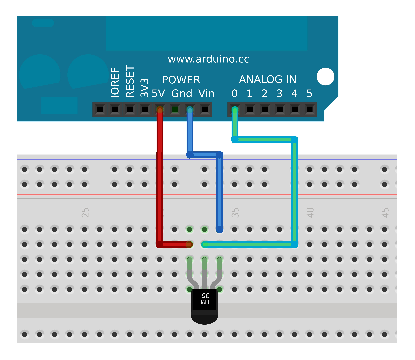
\includegraphics[width=0.7\linewidth]{figures/thermometer-fritzing.eps}
  \caption{Thermometer.}
  \label{fig:thermometer-fritzing}
\end{figure}

\begin{figure}[htbp]
  \centering
  \includegraphics[width=0.7\linewidth]{figures/thermometer-photo.eps}
  \caption{Thermometer.}
  \label{fig:thermometer-photo}
\end{figure}

\section{The code} 
Once inside, enter the following code:

\begin{lstlisting} [caption = {Blinking LED example code}, language = C, label = {code:blinkingLED}, numbers = left, escapeinside={@}{@}]
// Code from
// http://www.matbra.com/en/2012/09/23/sensor-de-temperatura-com-arduino-e-lm35-arduino-lm35/ 
int analogPin = 0; 
int readValue = 0; 
float temperature = 0; 
float temperatureF = 0;
void setup() { 
  Serial.begin(9600); 
}

void loop() { 
  readValue = analogRead(analogPin);
  //Serial.println(readValue);
  temperature = (readValue * 0.0049); 
  temperature = temperature * 100; 
  temperatureF = (temperature * 1.8) + 32;
  Serial.print("Temperature: "); 
  Serial.print(temperature); 
  Serial.print("C ");
  Serial.print(temperatureF);
  Serial.println("F");
  delay(1000); 
}
\end{lstlisting}

If you open the serial monitor, you should obtain results such as the ones in Fig.~\ref{fig:temperature-measures}.


\begin{figure}[htbp]
  \centering
  \includegraphics[width=0.7\linewidth]{figures/temperature-measures.eps}
  \caption{Thermometer.}
  \label{fig:temperature-measures}
\end{figure}

Try touching the thermometer with your finger and see how the temperature changes. What if you blow a little bit of cool air towards it?

\section{Next Steps}
There is not much networking in this thermometer now.
Let's send the data to a remote computer using an XBee.
